\documentclass[../Interim_Report_Master]{subfiles}
\begin{document}
\hypertarget{num_meth}{\section{Numerical Methods}\label{num_meth}}
Given the governing equations are coupled and non-linear finding an analytical solution has not proved possible. It is therefore necessary to use a numerical scheme to solve the equations. The choice of scheme and its implementation are especially important when considering the solution must work for millions of droplets. The scheme should of course be accurate but its complexity is also a consideration. There is no point choosing a method that is very accurate but is slow because the because this will be compounded greatly across millions of particles. In addition to this the method must be stable and resistant to non-physical phenomena. (I.e. the droplet mass cannot go below zero).

In terms of implementation the order in which the equations are solved may prove to be important. For example at a given time level should the temperature of the droplet be found before the mass? And what kind of error checking within the time step should take place?

Analytical solutions to the equations decoupled are available and provide a point of comparison for some of the schemes.

\subsection{Timestepping Procedure}
Numerical methods work by taking discrete steps forward in time. The length of the simulation is determined by the size of the timestep and the maximum number of timesteps. The timestepping procedure is shown in Figure \ref{timestep_proc}.

\begin{figure}
	\centering
	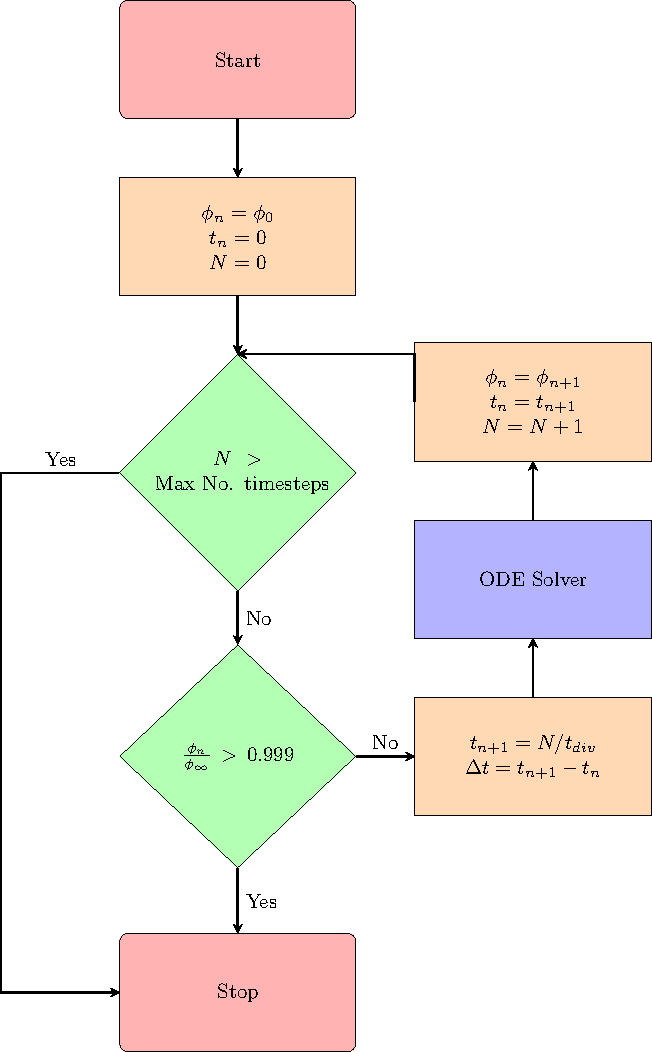
\includegraphics[width=0.5\textwidth]{./Diagrams/Timestepping_Procedure/Timestepping_Procedure.pdf}
	\caption{General timestepping procedure.}
	\label{timestep_proc}
\end{figure}

There are two conditions for the loop to run. The maximum number of time steps must not have been exceeded and the physical property $\phi$ cannot have converged to its value at infinity. This works for droplet temperature whilst for mass the condition would be a ratio of current to initial mass being greater than zero. Limiting the maximum number of time steps is necessary to prevent an infinite recursion in the case of the simulation being unable to converge. Also by specifying the value $t_{div}$ in addition to $N$ the size of time step and total time to be simulated is set.

The ODE solver is a black box that returns a numerical solution to the ODE at each discrete timestep. Some examples are given in the following subsections.

\subsection{Euler Method}
The simplest numerical method is to step forward in time and take the value at the next time level to be the current value plus a prediction on what the change between the values will be. This can be derived from the Taylor Series:
\begin{equation}
f(x+h) = f(x)+hf^\prime(x)+\frac{h^2}{2}f^{\prime\prime}(x)+..+\frac{h^{n-1}}{(n-1)!}f^{(n-1)}(x)+\frac{h^n}{n!}f^n(c)
\end{equation}

Using $\Delta t$ as $h$ and $a$ as the value at the current time level $n$, from the first two terms in the series:
\begin{equation}
f(n+1) = f(n)+\Delta tf^\prime(n)
\end{equation}

This is the forward Euler method and can be used to solve ODEs of the form:
\begin{equation}
\frac{d\phi}{dt} = f(t,~\phi)
\end{equation}

in increments of \(\Delta t\), by assuming for a small time step the output of the differential is constant. The formula is:
\begin{equation}
\phi_{n+1} = \phi_n + \Delta tf(t_n,~\phi_n)
\end{equation}

This formula is used in Figure \ref{timestep_proc} as the ODE solver:
\begin{figure}
	\centering
	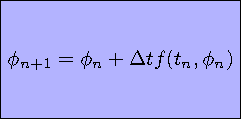
\includegraphics[width=0.4\textwidth]{./Diagrams/Forward_Euler_Method_Flowchart/Forward_Euler_Method_Flowchart.pdf}
	\caption{Forward Euler method solver.}
	\label{forward_euler}
\end{figure}

The forward Euler method is easy to start with only the initial conditions being required.

The order of the error can be found by again considering the Taylor series:
\begin{subequations}
\begin{eqnarray}
f(x+h) = f(x)+hf^\prime(x)+\frac{h^2}{2}f^{\prime\prime}(x) \\
f(x+h) = f(x)+hf^\prime(x)+O(h^2)
\end{eqnarray}
\end{subequations}

The $O(h^2)$ term is the local truncation error, the error inherited at each time step. Therefore, the local error is proportional to $h^2$. The order of the method is however of first order. I.e the error overall is proportional to $h$ since the number of steps is proportional to $1/h$. 

\subsection{Modified Euler Method}
The problem with the forward Euler method is it makes one prediction about what the solution will be at the next time step and assumes this solution is correct. This method can be modified so that the current and predicted value are used to estimate the gradient over the interval. This gives a more accurate numerical estimation of the gradient so the solution at the next time step should also be more accurate. 

Based on this the general formula is:
\begin{equation}
\phi_{n+1} = \phi_n+\frac{\Delta t}{2}\left[f(t_n,\phi_n)+f(t_{n+1},\tilde{\phi}_{n+1})\right]
\end{equation}

The term $f(t_{n+1},\phi_{n+1})$ is the prediction made using the forward Euler method. A flowchart representation of the method is shown in Figure \ref{mod_euler}. 
\begin{figure}
	\centering
	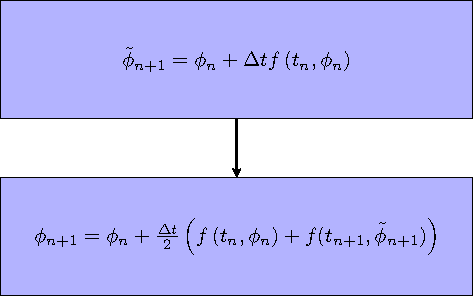
\includegraphics[width=0.5\textwidth]{./Diagrams/Modified_Euler_Method_Flowchart/Modified_Euler_Method_Flowchart.pdf}
	\caption{Modified Euler method solver.}
	\label{mod_euler}
\end{figure}

\subsection{Runge-Kutta Method}
The modified Euler method (also known as the Heun formula) is a predictor corrector method. In fact it is an example of a more general family of predictor corrector methods known as the Runge-Kutta method. The modified Euler method is in fact a second order Runge-Kutta method:
\begin{subequations}
\begin{eqnarray}
k_1 =& \Delta t f(t_n,\phi_n) \\
k_2 =& \Delta t f\left(t_n+\Delta t, \phi_n+k_1\right) \\
\phi_{n+1} =& y_n + \frac{1}{2}(k_1+k_2)
\end{eqnarray}
\end{subequations}	

The predictor corrector process can be extended such that 4 estimates of the solution are made, which are then averaged in a single formula. This gives a fourth order accurate scheme.
\begin{subequations}
\begin{eqnarray}
k_1 =& \Delta t f(t_n,\phi_n) \\
k_2 =& \Delta t f\left(t_n+\frac{\Delta t}{2}, \phi_n+\frac{k_1}{2}\right) \\
k_3 =& \Delta t f\left(t_n+\frac{\Delta t}{2}, \phi_n+\frac{k_2}{2}\right) \\
k_4 =& \Delta t f\left(t_n+\Delta t, \phi_n+k_3\right) \\
\phi_{n+1} =& \phi_n + \frac{1}{6}(k_1+2k_2+2k_3+k_4)
\end{eqnarray}
\end{subequations} 

More weighting is applied to the terms $k_2$ and $k_3$ as these are estimates of the midpoint of the interval. The procedure is shown in Figure \ref{runge_kutta}.
\begin{figure}
	\centering
	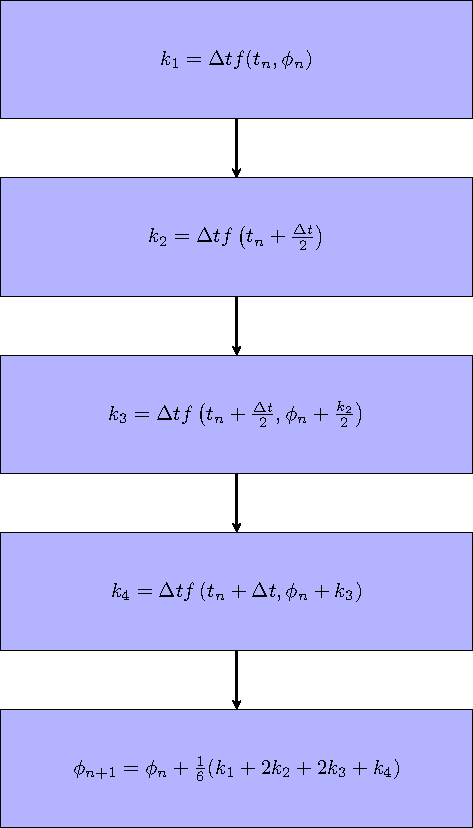
\includegraphics[width=0.5\textwidth]{./Diagrams/Runge_Kutta_Method_Flowchart/Runge_Kutta_Method_Flowchart.pdf}
	\caption{Flowchart for the Runge-Kutta method.}
	\label{runge_kutta}
\end{figure}

\subsection{Backward Euler Method}
The previously mentioned methods are all examples of explicit methods. So called as a function for the next value in time can be expressed explicitly in terms of known variables. The disadvantage of such methods is they extrapolate into the future; for small time steps this is fine as the error is small. But for larger time steps (relative to the timescale of the problem) this can cause instability and the solution diverges. 

An implicit method uses a function with $y_{n+1}$ on both the left and right hand side of the equation. In general this means an iterative method must be used to solve for $y_{n+1}$. However, for simpler equations an explicit function can be found. The benefit of an implicit method is it is in theory more stable than an explicit method.

A first order accurate implicit method is the backward Euler method:
\begin{subequations}
\begin{eqnarray}
t_{n+1} =& t_n + \Delta t \\
y_{n+1} =& y_n + \Delta t f(t_{n+1},y_{n+1})
\end{eqnarray}
\end{subequations} 

The general solution procedure using this method is shown in Figure x.

Figure x

A non-iterative formula can be derived for the temperature and mass ODES. Unlike the explicit methods, the implicit method will have to be derived for each ODE. For the temperature ODE:
\begin{equation}
\frac{dT_{d}}{dt} = \frac{f_{2}Nu}{3Pr_{G}}\left(\frac{\theta_1}{\tau_d}\right)(T_{G}-T_{d}) + \left(\frac{L_{V}}{C_{L}}\right)\frac{\dot{m}_{d}}{m_{d}} - H_{\Delta T}
\end{equation}

\begin{subequations}
\begin{align}
t_{n+1} =& \Delta t \\
T_{d_{n+1}} =& T_{d_{n}} + \Delta t \left[\frac{f_{2}Nu}{3Pr_{G}}\left(\frac{\theta_1}{\tau_d}\right)(T_{G}-T_{d_{n+1}}) + \left(\frac{L_{V}}{C_{L}}\right)\frac{\dot{m}_{d}}{m_{d}} - H_{\Delta T}\right]
\end{align}
\end{subequations} 

For the second equation rearrangement is required, the full process is shown in Section \ref{back_euler_temp_dev}:
\begin{subequations}
\begin{align}
T_{d_{n+1}} =& T_{d_{n}} + \Delta t \left[\frac{f_{2}Nu}{3Pr_{G}}\left(\frac{\theta_1}{\tau_d}\right)(T_{G}-T_{d_{n+1}}) + \left(\frac{L_{V}}{C_{L}}\right)\frac{\dot{m}_{d}}{m_{d}} - H_{\Delta T}\right] \\
T_{d_{n+1}} =& \frac{T_{d_{n}} + \Delta t \left[T_{G}\frac{f_{2}Nu}{3Pr_{G}}\left(\frac{\theta_1}{\tau_d}\right) + \left(\frac{L_{V}}{C_{L}}\right)\frac{\dot{m}_{d}}{m_{d}} - H_{\Delta T}\right]}{\left(1+\Delta t\frac{f_{2}Nu}{3Pr_{G}}\left(\frac{\theta_1}{\tau_d}\right)\right)} 
\end{align}
\end{subequations} 

A similar process can be applied to find an equivalent expression for the mass ODE:
\begin{equation}
\frac{dm_{d}}{dt} = -\frac{Sh}{3Sc_{G}}\left(\frac{m_{d}}{\tau_{d}}\right)H_M
\end{equation}

With:
\begin{subequations}
\begin{align}
t_{n+1} =& \Delta t \\
m_{d_{n+1}} =& m_{d_{n}} + \Delta t \left[-\frac{Sh}{3Sc_{G}}\left(\frac{m_{d_{n+1}}}{\tau_{d}}\right)H_M\right]
\end{align}
\end{subequations} 

Rearranging the second equation leads to:
\begin{equation}
m_{d_{n+1}} = \frac{m_{d_{n}}}{1+ \Delta t\frac{Sh}{3Sc_{G}}\left(\frac{H_M}{\tau_{d}}\right)} 
\end{equation} 

(The full solution can be found in Section \ref{back_euler_mass_dev}). These numerical methods will be evaluated in the next section to determine their suitability.

%\subsection{Central Difference Method}
%The Euler method is only first order accurate, halving the step size halves the error. A second order method has the property that if the step size is halved the error is reduced by a factor of four. A second order method could take an extra term from the Taylor series, but this requires differentiating the ODE. A less complicated method is to use first order terms to construct a method that is second order.
%
%The formula can again be found using a Taylor series expansion of $f(x)$:
%\begin{subequations}
%\begin{eqnarray}
%f(x+h) = f(x)+hf^\prime(x)+\frac{h^2}{2}f^{\prime\prime}(x) \\
%f(x-h) = f(x)-hf^\prime(x)+\frac{h^2}{2}f^{\prime\prime}(x)
%\end{eqnarray}
%\end{subequations}
%
%subtracting the previous two equations and neglecting higher (second) order terms gives:
%\begin{subequations}
%\begin{eqnarray}
%f(x+h) - f(x-h) = 2hf^\prime(x) \\
%f^\prime(x) = \frac{f(x+h) - f(x-h)}{2h} \\
%f(x+h) = f(x-h) + 2hf^\prime(x) \\
%y_{n+1} = y_{n-1} + 2\Delta tf(x_n,~y_n)
%\end{eqnarray}
%\end{subequations}

\end{document}